% paper/latex/figures/figure1_framework.tex
% Persona-CAPS framework schematic. Drop into main_body via % paper/latex/figures/figure1_framework.tex
% Persona-CAPS framework schematic. Drop into main_body via % paper/latex/figures/figure1_framework.tex
% Persona-CAPS framework schematic. Drop into main_body via % paper/latex/figures/figure1_framework.tex
% Persona-CAPS framework schematic. Drop into main_body via \input{figures/figure1_framework.tex}.
\begin{figure}[t]
\centering
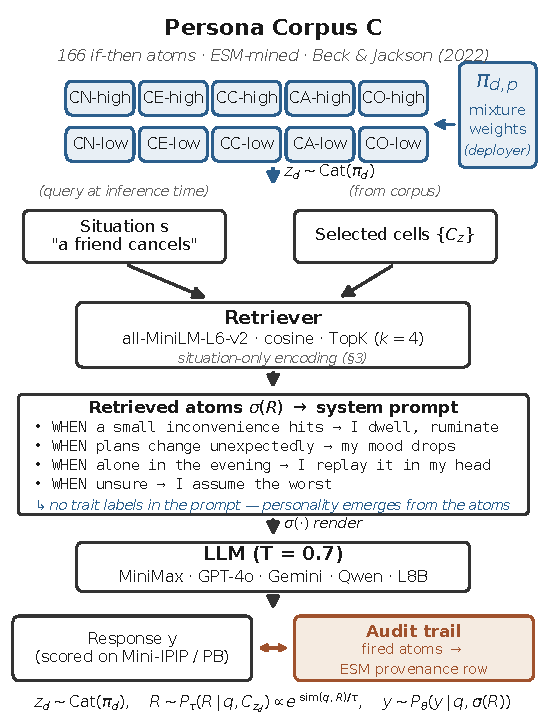
\includegraphics[width=\columnwidth]{figures/figure1_framework.pdf}
\caption{Persona-CAPS at inference. A persona is a corpus $C$ of \texttt{if-then} atoms organised into ten (dim, polarity) cells. Deployer-set mixture weights $\pi_{d,p}$ select active cells; the retriever encodes the query and each atom's situation field (\texttt{all-MiniLM-L6-v2}, cosine, top-$k{=}4$); retrieved atoms are rendered into a system prompt that contains \emph{no trait labels}; the LLM samples response $y$ at $T{=}0.7$; every fired atom is logged with provenance back to its ESM observation, yielding a per-response audit trail (\S~4.3). Conditional independencies, for a single dimension $d$ under control: $z_d \sim \mathrm{Cat}(\pi_d)$, $R \sim P_\tau(R \mid q, C_{z_d})$, $y \sim P_\theta(y \mid q, \sigma(R))$. The 5-D composition of \S~4.6 selects one $z_d$ per dimension and concatenates the five retrieved sets.}
\label{fig:framework}
\end{figure}
.
\begin{figure}[t]
\centering
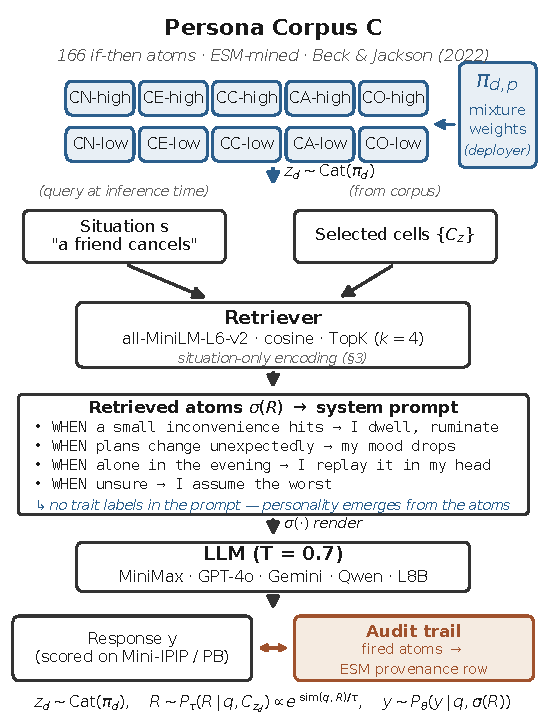
\includegraphics[width=\columnwidth]{figures/figure1_framework.pdf}
\caption{Persona-CAPS at inference. A persona is a corpus $C$ of \texttt{if-then} atoms organised into ten (dim, polarity) cells. Deployer-set mixture weights $\pi_{d,p}$ select active cells; the retriever encodes the query and each atom's situation field (\texttt{all-MiniLM-L6-v2}, cosine, top-$k{=}4$); retrieved atoms are rendered into a system prompt that contains \emph{no trait labels}; the LLM samples response $y$ at $T{=}0.7$; every fired atom is logged with provenance back to its ESM observation, yielding a per-response audit trail (\S~4.3). Conditional independencies, for a single dimension $d$ under control: $z_d \sim \mathrm{Cat}(\pi_d)$, $R \sim P_\tau(R \mid q, C_{z_d})$, $y \sim P_\theta(y \mid q, \sigma(R))$. The 5-D composition of \S~4.6 selects one $z_d$ per dimension and concatenates the five retrieved sets.}
\label{fig:framework}
\end{figure}
.
\begin{figure}[t]
\centering
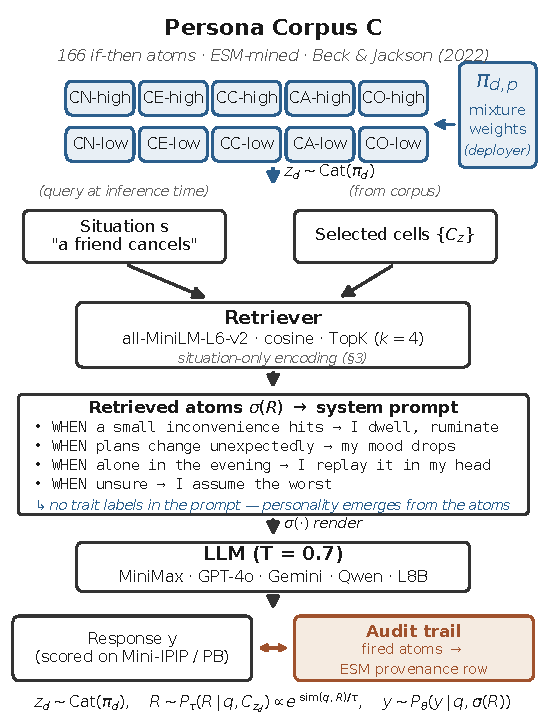
\includegraphics[width=\columnwidth]{figures/figure1_framework.pdf}
\caption{Persona-CAPS at inference. A persona is a corpus $C$ of \texttt{if-then} atoms organised into ten (dim, polarity) cells. Deployer-set mixture weights $\pi_{d,p}$ select active cells; the retriever encodes the query and each atom's situation field (\texttt{all-MiniLM-L6-v2}, cosine, top-$k{=}4$); retrieved atoms are rendered into a system prompt that contains \emph{no trait labels}; the LLM samples response $y$ at $T{=}0.7$; every fired atom is logged with provenance back to its ESM observation, yielding a per-response audit trail (\S~4.3). Conditional independencies, for a single dimension $d$ under control: $z_d \sim \mathrm{Cat}(\pi_d)$, $R \sim P_\tau(R \mid q, C_{z_d})$, $y \sim P_\theta(y \mid q, \sigma(R))$. The 5-D composition of \S~4.6 selects one $z_d$ per dimension and concatenates the five retrieved sets.}
\label{fig:framework}
\end{figure}
.
\begin{figure}[t]
\centering
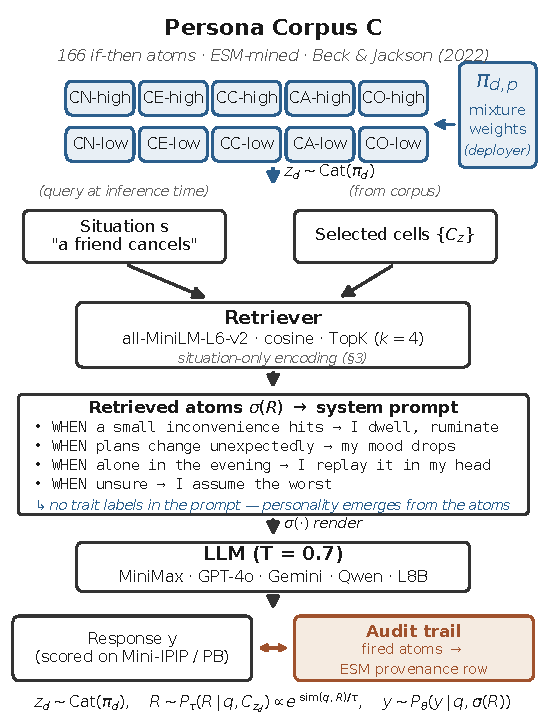
\includegraphics[width=\columnwidth]{figures/figure1_framework.pdf}
\caption{Persona-CAPS at inference. A persona is a corpus $C$ of \texttt{if-then} atoms organised into ten (dim, polarity) cells. Deployer-set mixture weights $\pi_{d,p}$ select active cells; the retriever encodes the query and each atom's situation field (\texttt{all-MiniLM-L6-v2}, cosine, top-$k{=}4$); retrieved atoms are rendered into a system prompt that contains \emph{no trait labels}; the LLM samples response $y$ at $T{=}0.7$; every fired atom is logged with provenance back to its ESM observation, yielding a per-response audit trail (\S~4.3). Conditional independencies, for a single dimension $d$ under control: $z_d \sim \mathrm{Cat}(\pi_d)$, $R \sim P_\tau(R \mid q, C_{z_d})$, $y \sim P_\theta(y \mid q, \sigma(R))$. The 5-D composition of \S~4.6 selects one $z_d$ per dimension and concatenates the five retrieved sets.}
\label{fig:framework}
\end{figure}
